\documentclass{beamer}
\usetheme{CambridgeUS}
\usecolortheme{beaver}
\usepackage{xeCJK}
\usepackage{hyperref}
\usepackage{tikz}
\usepackage{float}
\usetikzlibrary{graphs}
\usefonttheme[onlymath]{serif}
\begin{document}


\begin{frame}
    \title{关于高斯消元}
    \author{An\_Account}
    \begin{titlepage}
    \end{titlepage}
\end{frame}

\begin{frame}{AUOJ53 数一数}
    \begin{itemize}
        \item 有一个$n$行$m$列的$01$矩阵,对于每一列来说,第$i$行的格子为$1$的概率为$p_i$,每一列有且仅有一个$1$。
        \item 你可以选择一个初始位置$(x,y)$,然后每次移动到$(x-1,y+1),(x,y+1),(x+1,y+1)$这三个格子中的一个,直到$y = m$,你的最终得分为经过的格子的权值之和。记这个权值为$f(m)$。
        \item 给定$n$,求出当$m\rightarrow\infty$时,$\frac{f(m)}{m}$的期望。
        \item $n\leq 6$
    \end{itemize}
\end{frame}

\begin{frame}{AUOJ53 数一数}
    \begin{itemize}
        \item 如果$m$是有限的,并且矩阵已经确定好了,那么我们可以直接在整个矩阵上$dp$。记$dp[i][j]$表示从第一列开始走到第$i$行$j$列,能得到的最大分数。
        \item 显然对于一列来说,相邻的两行的$dp$值至多相差$1$。因此我们可以将当前列的$dp$值压成一个状态。通过爆搜状态可以得知,状态总数为$478$种。
        \item 同时,求出状态之间转移时对$f(m)$的影响,而$\frac{f(m)}{m}$本质上是求接下来的每次转移,使得当前$f$能$+1$的概率。
    \end{itemize}
\end{frame}

\begin{frame}{AUOJ53 数一数}
    \begin{itemize}
        \item 求出当$m\rightarrow\infty$时,每种状态出现的概率,那么我们就能够通过这个概率以及每种转移使得答案增加的概率算出$\frac{f(m)}{m}$。
        \item 钦定一种状态的出现频率为$1$,通过高斯消元解出所有状态的出现频率,然后用频率除以频率之和就得到了出现的概率。
    \end{itemize}
\end{frame}

\begin{frame}{(False)faces}
    \begin{itemize}
        \item 给出一张二分图,判断它的完美匹配个数模$4$是否为$0$。
        \item $n\leq 300$
    \end{itemize}
\end{frame}

\begin{frame}{(False)faces}
    \begin{itemize}
        \item 本质上是判断积和式的值模$4$是否为$0$。
        \item 介绍:来自论文的算法
        \item 首先我们有
        \item $$\begin{aligned}
            \operatorname{perm}A=(-1)^n\sum_{x\in\{0,1\}^n}(-1)^{x_1+x_2+\cdots +x_n}\prod_{i=1}^n(Ax)_i
        \end{aligned}$$
        \item 证明可以考虑容斥:枚举哪些行一定没有被选。
        \item 观察到式子中间有一个$\prod$,由于我们要求这个东西模$4$的余数,因此$(Ax)_i$至多只能有两个位置模$2$为$0$。
    \end{itemize}
\end{frame}

\begin{frame}{(False)faces}
    \begin{itemize}
        \item 我们有一个大胆的想法。
        \item 只考虑$(Ax)_i$每一项模$2$的余数,由于至多只能有一个$0$,因此我们可以枚举这个东西的取值,它只有$O(n)$种。
        \item 对于每种取值,通过高斯消元解出满足条件的所有$x$,再将每一组$x$代入刚刚的式子中求出答案。
        \item 问题是,合法的$x$的个数可能很大,直接解复杂度可能是指数级别的(需枚举自由元的取值)。
        \item 对这个矩阵做一些变换。
    \end{itemize}
\end{frame}

\begin{frame}{(False)faces}
    \begin{itemize}
        \item $$\left(\begin{matrix}
            A_{1,1} & A_{1,2} & \cdots & A_{1, n} & v_1 \\
            A_{2,1} & A_{2,2} & \cdots & A_{2, n} & v_2 \\
            \vdots  &         &        &          & \vdots\\
            A_{n,1} & A_{n,2} & \cdots & A_{n, n} & v_n \\
            0       & 0       & 0      & 0        & 1
        \end{matrix}\right)$$
        \item 这个矩阵的积和式等于原矩阵的积和式。
        \item 如果我们随机选取$v$,那么对于一个确定的$Ax$,每一组$x$成为它的解的概率为$\frac{1}{2^n}$。由于$x$一共有$2^n$种,因此此时对于每组$Ax$期望只有$O(1)$组解。
        \item 时间复杂度$O(n^4)$
    \end{itemize}
\end{frame}

\begin{frame}{来源不明的题}
    \begin{itemize}
        \item 给出一个二分图,两侧的点数分别为$n, m$,求完美匹配个数模$2$的余数。
        \item $n,m\leq 500$
    \end{itemize}
\end{frame}

\begin{frame}{来源不明的题}
    \begin{itemize}
        \item 不妨设$n<m$,那么我们将得到一个$n\times m$的邻接矩阵。
        \item 对这个矩阵进行类似消元的过程。\newline
        \begin{center}
            \begin{tikzpicture}
                \draw[->] (0.1, 0.1) rectangle (3.1, 1.6);
                \draw[dashed] (0, 0) rectangle (1.5, 1.5);
                \node(a) at (0.75, 0.75) {$I$};
            \end{tikzpicture}
        \end{center}
        \item 将虚线框住的部分消成单位矩阵,由于此时行列式的奇偶性可以看作从每行选出一个数,它们不同列的方案数,因此问题转化为对于未被框住的部分,选择若干个$1$,使得没有两个$1$同行或同列的方案数。
        \item 假设这个未被框住的矩阵为$A$。
    \end{itemize}
\end{frame}

\begin{frame}{来源不明的题}
    \begin{itemize}
        \item 我们构造一个这样的矩阵:\newline
        \begin{center}
            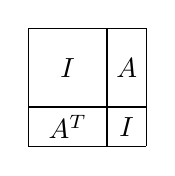
\begin{tikzpicture}
                \draw[] (0, 0) |- (1, 1);
                \draw[] (0, 0) -| (1, 1);
                \draw[] (1, 1) -| (1.5, -0.5);
                \draw[] (1, 0) -- (1.5, 0);
                \draw[] (0, 0) -| (1, -0.5);
                \draw[] (0, 0) |- (1.5, -0.5);
                \node(a) at (0.5, 0.5) {$I$};
                \node(b) at (1.25, 0.5) {$A$};
                \node(c) at (0.5, -0.25) {$A^T$};
                \node(d) at (1.25, -0.25) {$I$};
            \end{tikzpicture}
        \end{center}
        \item 容易发现假如从$A$中选出若干个不在同一行也不在同一列的$1$的方案数为$k$,那么这个矩阵的积和式的值就为$k^2$。
        \item 注意到$1^2\equiv 1\pmod 2, 0^2\equiv 0\pmod 2$。
        \item 在模$2$意义下,积和式的值等于行列式,因此直接对这个矩阵进行消元,当且仅当矩阵满秩时答案为$1$。
    \end{itemize}
\end{frame}

\begin{frame}{101221H Pachinko}
    \begin{itemize}
        \item 一个$n\times m$的棋盘,每个格子为". X T"三者之一,保证第一行没有T。现在在棋盘第一行的空位中等概率随机放一个球。
        \item 每当球到达一个新的空地时,它分别有$p_1\sim p_4$的概率往四个方向弹,如果弹跳会使得球碰到障碍物则球会被反弹,可以视为在原地重新进行一次随机。
        \item 当球进入T时游戏结束,问最终球滚入每个T的概率。
        \item $n\leq 10^4, m\leq 20$
    \end{itemize}
\end{frame}

\begin{frame}{101221H Pachinko}
    \begin{itemize}
        \item 对第$i$行$j$列的格子编号为$(i - 1)\times m + j$,所有格子的编号都在$1$到$n\times m$之间。
        \item 直接进行高斯消元复杂度为$O(n^3m^3)$,难以承受。
        \item 可以发现一个格子的方程只与它上下左右四个格子有关,因此整个矩阵应该是很稀疏的。换句话说,第$i$个方程中系数不为$0$的变量的下标在$[i - m, i + m]$之间。
    \end{itemize}
\end{frame}

\begin{frame}{101221H Pachinko}
    \begin{itemize}
        \item 考虑优化高斯消元的过程。
        \begin{figure}
            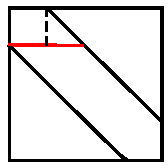
\includegraphics{1.pdf}
        \end{figure}
        \item 如果不考虑交换两行的情况,可以发现用第一行去消其它行时,只有前$m$行可能受到影响。
        \item 由于处理到第$i$行时前$i-1$位必然被前面的行消掉了,因此每次往后消元的时候只需枚举$m$行,且消元时只用消$[i, i + m]$这$m$个变量,时间复杂度$O(nm^3)$。
    \end{itemize}
\end{frame}

\begin{frame}{101221H Pachinko}
    \begin{itemize}
        \item 在普通的高斯消元中,如果$A_{i,i}=0$,那么我们需要找到一行满足$A_{j,i}\neq 0$,然后交换这两行。
        \item 注意到$A_{j,i}\neq 0$的$j$只可能在$[i, i+m]$中,交换这两行之后,第$i$行可能影响到的行仍然是$[i, i+m]$,但是消元时影响到的变量变成了$[i, i + 2 * m]$。
        \item 时间复杂度仍为$O(nm^3)$
    \end{itemize}
\end{frame}

\end{document}